\documentclass[12pt,a4paper,oneside]{article}
\usepackage[utf8]{inputenc}
\usepackage[english]{babel}
\usepackage{amsmath}
\usepackage{amsfonts}
\usepackage{amssymb}
\usepackage{graphicx}
\usepackage[]{algorithm2e}
\usepackage[left=2cm,right=2cm,top=2cm,bottom=2cm]{geometry}
%\usepackage{algorithm}
%\usepackage{algorithmic}

\begin{document}

\begin{center}
\textbf{\large{Report October 12th}} \\
%\textbf{Improving the formalization of the algorithm and Building our architecture}
\end{center}

\section{Formal definition of the Rhone service based query rewriting algorithm}

The basic input for the Rhone algorithm is: (1) a query; (2) a list of concrete services.
%In order to illustrate our definition let us suppose the following query example.
%Let us suppose the following query example in order to illustrate our definitions.

\noindent \textbf{Definition 1 (Query):} 
%A query $Q$ has the form:
A query $Q$ is defined as a set of \textit{abstract services}, a set of \textit{constraints}, and a set of \textit{user preferences} in accordance with the grammar: 
\begin{center}
$Q (\overline{I}, \overline{O}) := A_{1}(\overline{I}, \overline{O}), A_{2}(\overline{I}, \overline{O}), ..,  A_{n}(\overline{I}, \overline{O}),C_{1},C_{2}, .., C_{m}[P_{1},P_{2}, .., P_{k}]$
\end{center}  
The left side of the definition is called the \textit{head} of the query; and the right side is called the \textit{body}. 
$\overline{I}$ and $\overline{O}$ are a set of \textit{input} and \textit{output} parameters, respectively.
Input parameters in both sides of the definition are called \textit{head variables}.
In contrast, input parameters only in the query body are called \textit{local variables}.
%A query is expressed as set of abstract services ($A$) which specify abstract functions performed by the query.
%An abstract service is abstract function performed by the query. 
Abstract services ($A_{1}, A_{2}, .., A_{n}$) describes a set of basic service capabilities.
%Constraints over the \textit{input} or \textit{output} parameters are defined in $C$.
$C_{1}, C_{2}, .., C_{m}$ are constraints over the \textit{input} and/or \textit{output} parameters.
The user preferences (over the services) are signed in $P_{1}, P_{2}, .., P_{k}$. $C$ and $P$ are in the form $x \otimes constant$ such that $\otimes \in\lbrace \geq, \leq, =, \neq, <, >\rbrace$.

To illustrate the definition, let us suppose the set of abstract services in Table \ref{example1} and the Example 1.
%Let us suppose the following query example in order to illustrate the definition.

\begin{table}[h]
\center
\begin{tabular}{|p{7cm}|p{7cm}|}
\hline 
\textbf{\textit{Abstract Service}} & \textbf{\textit{Description}} \\ 
\hline 
\textit{DiseaseInfectedPatients(d?,p!)} & Given a disease \textit{d}, a list of patients \textit{p} infected by it is retrieved. \\ 
\hline 
\textit{PatientDNA(p?,dna!)} & Given a patient \textit{p}, his DNA information \textit{dna} is retrieved. \\ 
\hline 
\textit{PatientPersonalInformation(p?,info!)} & Given a patient \textit{p}, his personal information \textit{info} is retrieved. \\ 
\hline 
\end{tabular} \caption{Abstract services description}
\end{table}\label{example1}


\noindent \textbf{Example 1:} %Let us suppose the following simple query. 
\textit{The user wants to retrieve the DNA information from patients infected by the disease `K' using services that have availability higher than 99\%, price per call less than 0.2 dollars, and the total cost less then 1 dollar}.
%Query and concrete service are formally defined as follows.

The query which express the Example 1 according to the Definition 1 and the abstract services in Table \ref{example1} is specified below.
The decorations ? and ! are used to specify input and output parameters, respectively. 

\begin{center}
$Q (d?, dna!) := DiseaseInfectedPatients(d?, p!), PatientDNA(p?, dna!),$ \\
$d = ``K"[availability > 99\%, \ price \ per \ call < 0.2\$, \ total \ cost < 1\$]$
\end{center}  

Analyzing the query, it is possible to note that the parameters ``d?'' and ``dna!'' appear in both sides of the definition.
Due to that they are \textit{head} variables.
On the other hand, ``p!'' and ``p?'' are \textit{local} variables considering that they appear only in the body definition. 
Additionally, note that the local variables ``p!'' and ``p?'' have the same name.
Intuitively, this fact indicates a dependency between the abstract services which use these variables (in that case \textit{DiseaseInfectedPatients} and \textit{PatientDNA}).

In the example, \textit{DiseaseInfectedPatients} and \textit{PatientDNA} are abstract services that specify basic service functions which are combined to answer the query. 
%\textit{DiseaseInfectedPatients} retrieves the patients infected by a given disease.
%\textit{PatientDNA} retrieves that DNA information of a patient.
The constraint ($d = ``K''$) over the input parameter `d' will be further used while executing the query over a database (the where clause). 
\textit{Availability}, \textit{price per call} and \textit{total cost} are the user preferences over the services.

\noindent \textbf{Definition 2 (Concrete service):} A concrete service ($S$):
\begin{center}
$S (\overline{I}, \overline{O}) := A_{1}(\overline{I}, \overline{O}), A_{2}(\overline{I}, \overline{O}), ..,  A_{n}(\overline{I}, \overline{O})[P_{1},P_{2}, .., P_{k}]$
\end{center}  
A concrete service ($S$) is defined as a set of abstract services ($A$), and by its quality constraints $P$. 
These quality constraints associated to the service represent the service level agreement exported by the concrete service.

\noindent \textbf{Example 2:} Considering the query (see Example 1) and the abstract services (see Table \ref{example1}), the concrete services below are examples in accordance with the Definition 2.

\begin{flushleft}
$S1 (a?, b!) := DiseaseInfectedPatients(a?, b!)[availability > 99\%, \ price \ per \ call = 0.2\$]$ \\
$S2 (a?, b!) := DiseaseInfectedPatients(a?, b!)[availability > 99\%, \ price \ per \ call = 0.1\$]$ \\
$S3 (a?, b!, c!) := DiseaseInfectedPatients(a?, b!, c!)[availability > 98\%, \ price \ per \ call = 0.1\$]$ \\
$S4 (a?, b!) := PatientDNA(a?, b!)[availability > 99.5\%, \ price \ per \ call = 0.1\$]$ \\
$S5 (a?, b!) := PatientDNA(a?, b!)[availability > 99.7\%, \ price \ per \ call = 0.1\$]$ \\
$S6 (a?, b!) := PatientPersonalInformation(a?, b!)[availability > 99.7\%, \ price \ per \ call = 0.1\$]$ \\
$S7 (a?, b!) := PatientDNA(a?, c!),PatientPersonalInformation(c?, b!)[availability > 99.7\%, \ price \ per \ call = 0.1\$]$ \\
\end{flushleft}

Given the query and a list of concrete services as input, the algorithm looks for candidate concrete services. 
Candidate concrete service is a concrete service that probably can be used in the rewriting process. 
It contains only abstract services which are also query abstract services, and with the same signature (same name and number of input/output variables).
The candidate concrete services are chosen while searching for matches between abstract services in $S$ and abstract service in $Q$. 
%The following definitions will guide us while selecting candidate concrete services.

\noindent \textbf{Definition 3 (abstract service equivalence):} 
A match between abstract services occurs when an abstract service $A_{i}$ is equivalent to $A_{j}$, denoted $A_{i} = A_{j}$. 
Given two abstract services $A_{i}$ and $A_{j}$, $A_{i}$ = $A_{j}$ iff: (1) $A_{i}$ and $A_{j}$ have the same abstract function name; (2) the number of \textit{input} parameters of $A_{i}$ is equal to $A_{j}$; and (3) the number of \textit{output} parameters of $A_{i}$ is equal to $A_{j}$. 
For example, looking to the concrete services in the Example 2, the abstract service \textit{DiseaseInfectedPatients} in $S1$ and $S2$ are equivalent to the abstract service \textit{DiseaseInfectedPatients} in the query $Q$ (Example 1) once they have the same name and number of input/output parameters.
On the other hand, the abstract service \textit{DiseaseInfectedPatients} in $S3$ is not equivalent to the abstract service \textit{DiseaseInfectedPatients} in the query because the number of parameters are different.

%\noindent \textbf{Definition 3 (Abstract service equivalence):} Given a query $Q$; a concrete service $S$; and an abstract service $A_{i}$ such that $A_{i} \in Q$ and $A_{i} \in S$, $A_{i}.Q$ is equivalent to $A_{i}.S$, denoted $A_{i}.Q = A_{i}.S$, iff the number of variables of $A_{i} \in Q$ is equal to the number of variables of $A_{i}.S$.

%Once a matching between abstract services is found, the algorithm checks if the concrete service associated in the matching is a candidate to be part of the rewriting process.

Based on the assumptions that: (a) a concrete service can represent a service composition in which the abstract services involved may be able not only to retrieve data, but also to execute business rules that may impact the entire system; and (b) the execution of a concrete service consists in executing all its abstract services.  
A concrete service (S) is selected as \textit{candidate} to the rewriting process if for each abstract service in $S$ there is an equivalent in $Q$; there is no abstract service in $S$ that does not exist in $Q$; and the quality constrains in $Q$ must be guaranteed in $S$.

\noindent \textbf{Definition 4 (candidate service):} Given a query $Q$ and a concrete service $S$, $S$ is a \textit{candidate} service iff: (1) $\nexists A_{i} \ s.t. \ A_{i} \in S \ and \ A_{i} \not\in Q$; and (2) the quality constraints in $S$ does not violate the user preferences in $Q$. 

For example, considering the query in the Example 1 and the concrete services in the Example 2, it is possible to see that:
%\begin{itemize}
%\item S1 and S3 are not a candidate services because they violate the user preferences.
(1) $S1$ is not a candidate service because it violates an user preference (\textit{price per call});
(2) $S3$ and $S7$ are not a candidate service because they have abstract services that are not in $Q$; and
(3) $S2$, $S4$ and $S5$ are candidate services once: all their abstract services have an equivalent in $Q$ and there is no violation in the user preference.
%\end{itemize}

%\noindent \textbf{Definition 4 (Candidate service):} Given a query $Q$ and a concrete service $S$, $S$ is a candidate service iff $\nexists A_{i} \ s.t. \ A_{i} \in S \ and \ A_{i} \not\in Q$. $\forall A_{i} \in S$ and an abstract service $A_{i}$ such that $A_{i} \in Q$ and $A_{i} \in S$, the mapping $A_{i}.Q \longmapsto A_{i}.S$ can be generated iff:
%(1) $A_{i}.Q = A_{i}.S$; and (2) $\nexists A \ s.t. \ A \in S \ and \ A \not\in Q$.

%In the next step, the algorithm builds the \textit{partial descriptors} (PD). 
%Each descriptor describes how a \textit{candidate} concrete service can be used in the query rewriting process.

%An important concept in our approach is the \textit{candidate service description} (CSD). 
A \textit{candidate service description} (CSD) describes how a \textit{candidate} concrete service can be used in the query rewriting process.
It is a complex data structure which includes: mappings from variables in a concrete service to variables in the query; 
mappings from variables on the head of a concrete service to variables on its body;
a set of abstract services that represents partially or fully the abstract services in the query; and 
a set of quality constrains associated to the concrete service.
Intuitively, a rewriting is a set of \textit{candidate service descriptions} that fully covers the original query, and do not violates the user preferences.

\noindent \textbf{Definition 5 (candidate service description):} A CSD is represented by an n-tuple: %follows: 
\begin{center}
$\langle S, h, \varphi, G, P\rangle$
\end{center}
where $S$ is a concrete service. 
\textit{h} are mappings between variables in the head of $S$ to variables in the body of $S$. 
$\varphi$ are mapping between variables in the concrete service to variables in the query.
$G$ is a set of abstract services covered by $S$. 
$P$ is a set quality constraints associated to the service $S$. 

The CSD for a given service will be created following rules: (1) for all head variables in $S$, there is a mapping for a head variable in $Q$; and (2) if $x$ is an local variable in $S$ mapped to a local variable in $Q$, then $S$ must cover all abstract services in $Q$ which uses $x$ or cover only one abstract service that uses $x$.

\noindent \textbf{Example 3:} To illustrate the rules above consider the following example. 
\textit{The user wants to retrieve the personal information and the DNA information from patients infected by disease ``K"}.
Supposing we have the query $Q$ and the concrete services $S1$, $S2$, $S3$ and $S4$:

\begin{center}
$Q (d?, info!, dna!) := DiseaseInfectedPatients(d?, p!), PatientDNA(p?, dna!), PatientPersonalInformation(p?, info!)$ \\
$S1 (a?, b!) := DiseaseInfectedPatients(a?, c!), PatientDNA(c?, b!)$ \\
$S2 (a?, b!) := PatientPersonalInformation(a?, b!)$ \\
$S3 (a?, b!) := DiseaseInfectedPatients(a?, b!)$ \\
$S4 (a?, b!) := PatientDNA(a?, b!)$ \\
\end{center} 

In the query $Q$ it is possible to note that ``p!'' is a \textit{local} variable which is used as input (``p?'') for the abstract services $A2$ and $A3$. 
Looking to the concrete service $S1$ no CSD will be created for it because the \textit{local} variable $c!$ is mapped to the local variable $p!$, but $S1$ does not cover all abstract services which expects that variable. 
On the other hand, CSDs are constructed to the services $S2$, $S3$ and $S4$ once even existing the mapping from a local variable in the concrete service to a local variable in the query, all of them only cover one abstract service which uses that \textit{local} variable.
To be more clear about these rules, consider the rewriting below in which the CSDs for the services  $S2$, $S3$ and $S4$ are used:

\begin{center}
$Q (d?, info!, dna!) := S3(d?, p!), S4(p?, dna!), S2(p?, info!)$ \\
\end{center}  

The rewriting above is the only one possible for the query. 
However, let us suppose that a CSD for $S1$ was created violating the rule number two, consequently the wrong rewriting below would be created:

\begin{center}
$Q (d?, info!, dna!) := S1(d?, info!),S4(p?, dna!)$ \\
\end{center}  

The problem here is regarding the \textit{local} variable $p?$ which appears in $S4$, and it apparently should come from $S1$, but we can not guarantee that the same \textit{local} variable internally used in $S1$ is the one expected by $S4$. 
That is the reason the rule two exists.

%\begin{flushleft}
%\textbf{Architecture}
%\end{flushleft}
%
%\textit{Query Generator Module} helps the user to create his queries, and to define his preferences. 
%Once we have a query this module will try to find if there are previous rewritings to a equivalent query. 
%If true, \textit{the composition and execution module} can publish and execute the new composition retrieving and integrating the new data.
%If there are no previous rewritings, the module interacts with the \textit{service locator} in order to identify in our \textit{service registry} services that can answer the query or part of it.
%The query and the selected services are used in the \textit{Query Rewriting Module} to generate the rewritings for the query. 
%The rewritings are sent to \textit{the composition and execution module} to be published and executed (perhaps we can use BPEL to compose and execute).
%The integration process could be done in our database or in the database of one related services (somehow we should analyze which one is the best option).
%
%\begin{figure}[h]
%\center
%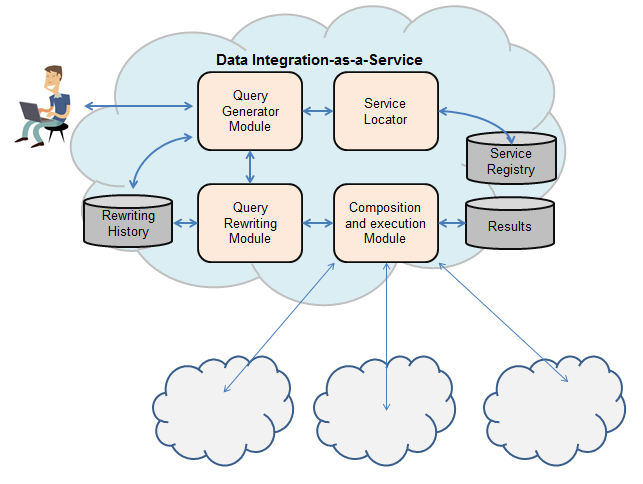
\includegraphics[scale=0.8]{arch.PNG} 
%\end{figure}


%-------------
% 
%A concrete service ($S$) is defined as a set of abstract services ($A$), and by its quality constraints $P$. 
%These quality constraints associated to the service represent the service level agreement exported by the concrete service.
%
%
%The \textbf{input data} for the algorithm is a query (Q) and a list of concrete services (C1, C2, ...). The query and concrete services are defined as follows:
%
%
%\begin{figure}[h]
%\center
%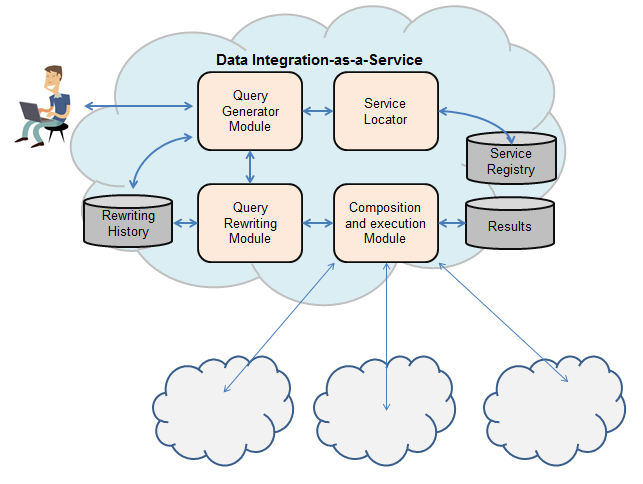
\includegraphics[scale=0.8]{arch.PNG} 
%\end{figure}
%
%
%
%The query and concrete services are defined as a set of abstract services ($A_{1}, A_{2}, ..., A_{n}$) and a set of quality constraints ($Q_{1},Q_{2}, ..., Q_{n}$). $\overline{t}$ is a set of input (decoration \textbf{?}) or output (decoration \textbf{!}) variables. The first \textbf{processing step} of the algorithm creates the data structures that represent the query and concrete services. The query and concrete service data structure will be formed by its $name$, a set of head variables ($V_{h}$) and a set of abstract services ($A_{s}$).
%
%\begin{center}
%$Q = \langle name, V_{h}, A_{s} \rangle$ \\
%$C = \langle name, V_{h}, A_{s} \rangle$
%\end{center}
%
%For each abstract service A in the set $A_{s}$, a data structure containing its $name$ and a set of variables ($V$) is build. Notice that the set of variables ($V$) can contain head variables or local variables.
%
%\begin{center}
%$A = \langle name, V\rangle$
%\end{center}
%
%Once these structures were created, the \textbf{second step in the algorithm is to form the PCDs}. PCDs are created only for those concrete services which have abstract services that can answer that query or part of it. PCDs are defined as follows:
%
%\begin{center}
%$\langle S, h, \varphi, G, Def, has\_opt\rangle$
%\end{center}
%
%\textbf{\textit{S}} is a concrete service. \textit{h} are mapping between terms in the head of the service definition to terms in the right side of the service definition. \textbf{\textit{$\varphi$}} are mapping between terms from the abstract composition to terms in the concrete service definition. \textbf{\textit{G}} is a set of abstract services names and quality constraints covered by \textbf{\textit{S}}. \textbf{\textit{Def}} is a set conditions that are not covered by \textbf{\textit{S}} alone.\textbf{ \textit{has\_opt}} is a boolean flag to indicate that some abstract service in the definition of \textbf{\textit{S}} has been used in \textbf{\textit{G}} and has an optional parameter.
%
%After that, all the \textbf{PCDs formed in the previous step are combined}. Once we have all the possible combinations of PCDs, \textbf{each combination is verified} to confirm if the combination is a valid rewriting of the former query or not.
%A valid rewriting is a list of PCDs that answers the complete query without redundancies, and without more than one mapping to the same variable with distinct values.
%\bigskip
%Considering that we have the data structure for the query (Q) and concrete services (C), the general idea of the algorithm is defined in the function \emph{rewriting}:
%
%\begin{verbatim}
%function rewriting (Q, C)
%   l := createPCDs(Q, C)
%   P := combinePCD (l)
%foreach p in P
%   if isRewriting(Q,p)
%      R := R U {p}
%return R
%\end{verbatim}
%
%\begin{algorithm}[H]
% \KwData{this text}
% \KwResult{how to write algorithm with \LaTeX2e }
% initialization\;
% \While{not at end of this document}{
%  read current\;
%  \eIf{understand}{
%   go to next section\;
%   current section becomes this one\;
%   }{
%   go back to the beginning of current section\;
%  }
% }
% \caption{How to write algorithms}
%\end{algorithm}
%
%
%The function \emph{createPCDs} returns a list of PCDs \textbf{l}. \textbf{P} is a list all possible combinations of PCDs returned by the function \emph{combinePCD}. And, for each PCD combination in \textbf{P}, the function \emph{isRewriting} verifies the combination is a valid rewriting or not. If true, the set of rewriting \textbf{R} is updated adding the new combination. In the end, the list of rewriting \textbf{R} is returned.
%
%\bigskip The examples next show the data structure created for input data, the intermediary data generated while processing the algorithm, and the output rewriting expected.
% 
%\begin{flushleft}
%\textbf{Describing an example 1}
%\end{flushleft}
%
%\begin{flushleft}
%\textbf{Query:} \\
%Q(disease?, patients!, dnas!, birth!, gen!, addr!, wheatherstatistic!) :- A1(disease?, patients!), A2(patients?,dnas!), A3(patients?, birth!, gen!, addr!), A4(addr?, wheatherstatistic!) \\
%\end{flushleft}
%
%The data created for the query above is:
%
%\begin{center}
%$\langle Q, [disease?, patients!, dnas!, birth!, gen!, addr!, wheatherstatistic!], [A1,A2,A3,A4] \rangle$
%\end{center}
%
%For each abstract service the following data is created:
%
%\begin{flushleft}
%$\langle A1, [disease?, patients!]\rangle$ \\
%$\langle A2, [patients?,dnas!]\rangle$ \\
%$\langle A3, [patients?, birth!, gen!, addr!]\rangle$ \\
%$\langle A4, [addr?, wheatherstatistic!]\rangle$ \\
%\end{flushleft}
%
%The same procedure is done for the concrete services.
%
%\begin{flushleft}
%\textbf{Concrete services:} \\
%S1(d?, p!) :- A1(d?, p!)\\
%S2(d?, p!) :- A1(d?, p!)\\
%S3(p?, d!) :- A2(p?, d!)\\
%S4(p?, dateofbirth!, gender!, address!) :- A3(p?, dateofbirth!, gender!, address!)\\
%S5(address?, wheatherstaticalinformation!) :- A4(address?, wheatherstaticalinformation!)\\
%S6(p?, d!) :- A5(p?, d!)\\
%S7(p?, vaccinateddiseases!) :- A6(p?, vaccinateddiseases!)\\
%\end{flushleft}
%
%Once we have all the data structure created, PCDs for abstract services that can solve the query will be created. Such as:
%
%\begin{flushleft}
%$\langle S1, [d? \longmapsto d?, p! \longmapsto p!], [d? \longmapsto disease?, p! \longmapsto patients!], A1, \emptyset, false\rangle$ \\
%$\langle S2, [d? \longmapsto d?, p! \longmapsto p!], [d? \longmapsto disease?, p! \longmapsto patients!], A1, \emptyset, false\rangle$ \\
%$\langle S3, [p? \longmapsto p?, d! \longmapsto d!], [p? \longmapsto patients?, d! \longmapsto dnas!], A2, \emptyset, false\rangle$ \\
%$\langle S4, [p? \longmapsto p?, dateofbirth! \longmapsto dateofbirth!, gender! \longmapsto gender!, address! \longmapsto address!], [p? \longmapsto patients?, dateofbirth! \longmapsto birth!, gender! \longmapsto gen!, address! \longmapsto addr!], A3, \emptyset, false\rangle$ \\
%$\langle S5, [address? \longmapsto address?, wheatherstaticalinformation! \longmapsto wheatherstaticalinformation!], [address? \longmapsto addr?, wheatherstaticalinformation! \longmapsto wheatherstatistic!], A4, \emptyset, false\rangle$ \\
%\end{flushleft}
%
%Based on these PCDs, all possible combination are created, and then the valid ones are returned as rewriting of the former query. The expected \textbf{rewriting results} are:
%
%\begin{flushleft}
%\textbf{1) }Q(disease,patients,dnas,birth,gen,addr,wheatherstatistic) :- S1(disease,patients),S3(patients,dnas),S4(patients,birth,gen,addr),S5(addr,wheatherstatistic) \\
%\textbf{2) }Q(disease,patients,dnas,birth,gen,addr,wheatherstatistic) :- S2(disease,patients),S3(patients,dnas),S4(patients,birth,gen,addr),S5(addr,wheatherstatistic) \\
%\end{flushleft}
%
%\begin{flushleft}
%\textbf{Describing an example 2}
%\end{flushleft}
%
%The difference between the example 1 and 2 is the concrete service S2. Now, I defined it being able to solve two parts in the query.
%
%\begin{flushleft}
%\textbf{Query:} \\
%Q(disease?, patients!, dnas!, birth!, gen!, addr!, wheatherstatistic!) :- A1(disease?, patients!), A2(patients?,dnas!), A3(patients?, birth!, gen!, addr!), A4(addr?, wheatherstatistic!) \\
%\end{flushleft}
%
%\begin{flushleft}
%\textbf{Concrete services:} \\
%S1(d?, p!) :- A1(d?, p!)\\
%S2(d?, p!, dna!) :- A1(d?, p!), A2(p?, dna!)\\
%S3(p?, d!) :- A2(p?, d!)\\
%S4(p?, dateofbirth!, gender!, address!) :- A3(p?, dateofbirth!, gender!, address!)\\
%S5(address?, wheatherstaticalinformation!) :- A4(address?, wheatherstaticalinformation!)\\
%S6(p?, d!) :- A5(p?, d!)\\
%S7(p?, vaccinateddiseases!) :- A6(p?, vaccinateddiseases!)\\
%\end{flushleft}
%
%Note the difference in the PCD for S2 in the following lines. Now the set \textbf{G} has indications for A1 and A2.
%
%\begin{flushleft}
%$\langle S1, [d? \longmapsto d?, p! \longmapsto p!], [d? \longmapsto disease?, p! \longmapsto patients!], A1, \emptyset, false\rangle$ \\
%$\langle S2, [d? \longmapsto d?, p! \longmapsto p!, dna! \longmapsto dna!], [d? \longmapsto disease?, p! \longmapsto patients!, dna! \longmapsto dnas!], \lbrace A1,A2 \rbrace, \emptyset, false\rangle$ \\
%$\langle S3, [p? \longmapsto p?, d! \longmapsto d!], [p? \longmapsto patients?, d! \longmapsto diseases!], A2, \emptyset, false\rangle$ \\
%$\langle S4, [p? \longmapsto p?, dateofbirth! \longmapsto dateofbirth!, gender! \longmapsto gender!, address! \longmapsto address!], [p? \longmapsto patients?, dateofbirth! \longmapsto birth!, gender! \longmapsto gen!, address! \longmapsto addr!], A3, \emptyset, false\rangle$ \\
%$\langle S5, [address? \longmapsto address?, wheatherstaticalinformation! \longmapsto wheatherstaticalinformation!], [address? \longmapsto addr?, wheatherstaticalinformation! \longmapsto wheatherstatistic!], A4, \emptyset, false\rangle$ \\
%\end{flushleft}
%
%Based on these PCDs, the expected \textbf{rewriting results} are:
%
%\begin{flushleft}
%\textbf{1) }Q(disease,patients,dnas,birth,gen,addr,wheatherstatistic) :- S1(disease,patients),S3(patients,dnas),S4(patients,birth,gen,addr),S5(addr,wheatherstatistic) \\
%\textbf{2) }Q(disease,patients,dnas,birth,gen,addr,wheatherstatistic) :- S2(disease,patients,dnas),S4(patients,birth,gen,addr),S5(addr,wheatherstatistic) \\
%\end{flushleft}


\end{document}